%%%%%%%%%%%%%%%%%%%%%%%%%%%%%%%%%%%%%%%%%%%%%%%%%%%
%
%  New template code for TAMU Theses and Dissertations starting Fall 2012.  
%  For more info about this template or the 
%  TAMU LaTeX User's Group, see http://www.howdy.me/.
%
%  Author: Wendy Lynn Turner 
%	 Version 1.0 
%  Last updated 8/5/2012
%
%%%%%%%%%%%%%%%%%%%%%%%%%%%%%%%%%%%%%%%%%%%%%%%%%%%
%%%%%%%%%%%%%%%%%%%%%%%%%%%%%%%%%%%%%%%%%%%%%%%%%%%%%%%%%%%%%%%%%%%%%%
%%                           SECTION V
%%%%%%%%%%%%%%%%%%%%%%%%%%%%%%%%%%%%%%%%%%%%%%%%%%%%%%%%%%%%%%%%%%%%%


\chapter{\uppercase{Experiments \& Results}}
To verify the idea proposed in this thesis, we setup experiment environments, develop SAC framework and run some typical seismic applications on cluster in PVAMU cloud computing lab. There are three main layers in SAC: low-level runtime environment, SAC framework as middleware and application development interface at up-level. Middleware layer of SAC was already discussed in pervious chapter. Runtime environments is the basic that SAC built on, and the application development interface is entry of user, which will be introduced respectively in the following sections.

\section{Experiments Environment Setup}

The cluster used for conducting experiments consists of 26 nodes, in which one is management node, another is storage node used for managing disk array and other 24 nodes are computation nodes. Each node in such cluster was equipped with Intel Xeon E5-2640 Sandy Bridge CPU (2.5GHz, 12 Cores or 24 Cores with Hyper-threading support), 64GB DDR3 memory and are inter-connected with 1GB ethernet. Each node has its own local disk, and also could access disk array through NFS. Following the architecture stated in previous chapter, we install CentOS 6.5 (Distributed by Redhat) and Oracle JDK 1.8.0\_40 on each node. Hadoop 2.2.0, Spark 1.2.1 (update to Spark 1.4.0 late) and other related libraries are also installed on each node. In configuration of Hadoop, management node was configured as NameNode and other 24 computation nodes as DataNodes. It is similar in Spark: management node is Master and other computation nodes are Workers. Cassandra was installed on all 24 computation nodes and the first four nodes of them was selected as seed nodes.

The public sample seismic dataset Penobscot \cite{PenobscotData} was selected as experiment data. The original format of Penobscot dataset is SEGY, and to make it easily processed with Spark, we transfer it into two files: one xml file that saves meta data, and another 3D data file with dimension size of 600x481x1501 stores actual data samples. The volume size of original data file is about 1.7GB, which is not big enough comparing with datasets currently used in oil \& gas industry, so we use it synthesize a new 100GB file for verifying algorithms and models on SAC. For some extensive time consuming algorithms, we still use 1.7GB file as test data. Both xml file and data file are stored on HDFS, so that every node could access them and utilize data locality. The intermediate results are stored in Cassandra basing on requirement and final result are persisted back to HDFS. 

\section{Application Development Platform}

As stated in previous chapter, user could create new application that calls APIs provided by SAC framework directly, but another more convenient way is using Web interface provide by SAC platform. In web development interface, SAC platform provides four main components: Projects, Data Sets, Jobs and Workflow. The typical flow is listed below:

\begin{enumerate}
  \item Create a project or open an existing project. While creating new project, user need to select template as shown in Figure \ref{NewProject}.
  \item Edit codes, compile project and fix errors until compiling successfully as shown in Figure \ref{Programming}.
  \item Select data set(s) as input parameter as shown in Figure \ref{DataSet}.
  \item Configure runtime environments and submit job to Spark Jobserver as shown in Figure \ref{Runtime}.
  \item Check job status and view results after job finished.
\end{enumerate}

%%%%%%%%%%%%%%%%%%%%%%%%%%%%%%%%%%%%%%%%%%%%%%%%%%%%%%%
\begin{figure}[h]
\centering
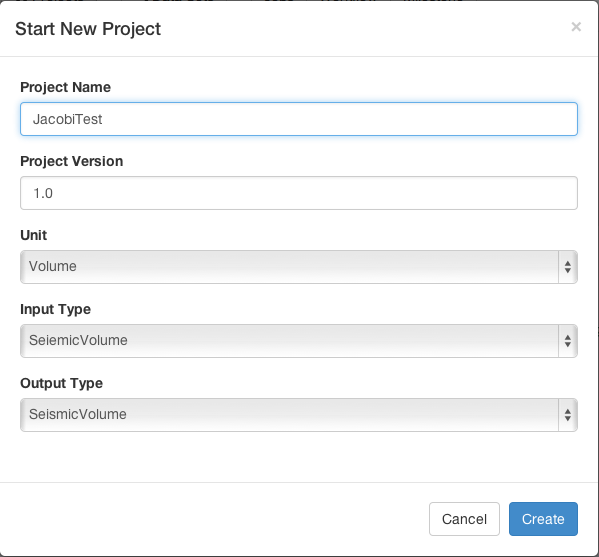
\includegraphics[scale=.60]{figures/NewProject.png}
\caption{Configure Template on Creating New Project}
\label{NewProject}
\end{figure}
%%%%%%%%%%%%%%%%%%%%%%%%%%%%%%%%%%%%%%%%%%%%%%%%%%%%%%%

%%%%%%%%%%%%%%%%%%%%%%%%%%%%%%%%%%%%%%%%%%%%%%%%%%%%%%%
\begin{figure}[h]
\centering
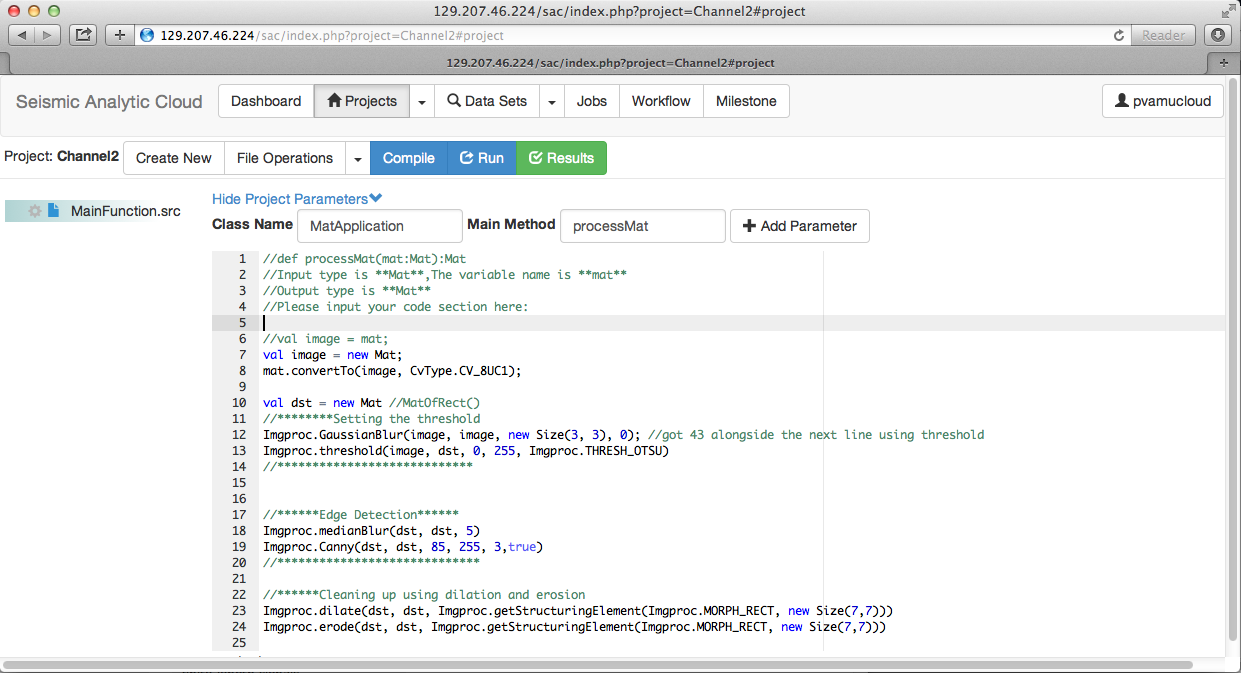
\includegraphics[scale=.35]{figures/Programming.png}
\caption{Programming and Running on Web Interface}
\label{Programming}
\end{figure}
%%%%%%%%%%%%%%%%%%%%%%%%%%%%%%%%%%%%%%%%%%%%%%%%%%%%%%%


%%%%%%%%%%%%%%%%%%%%%%%%%%%%%%%%%%%%%%%%%%%%%%%%%%%%%%%
\begin{figure}[h]
\centering
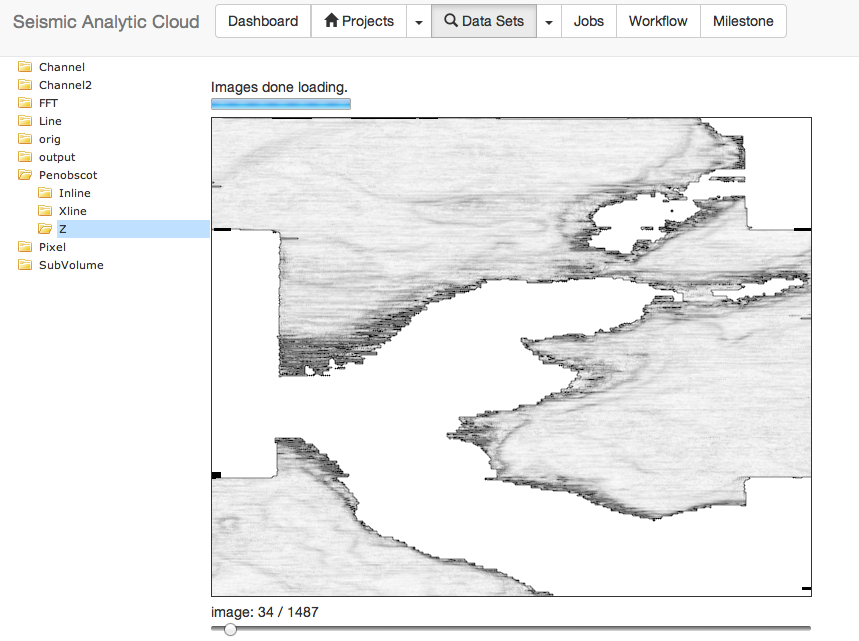
\includegraphics[scale=.45]{figures/DataSet.png}
\caption{Seismic Dataset Preview}
\label{DataSet}
\end{figure}
%%%%%%%%%%%%%%%%%%%%%%%%%%%%%%%%%%%%%%%%%%%%%%%%%%%%%%

%%%%%%%%%%%%%%%%%%%%%%%%%%%%%%%%%%%%%%%%%%%%%%%%%%%%%%%
\begin{figure}[h]
\centering
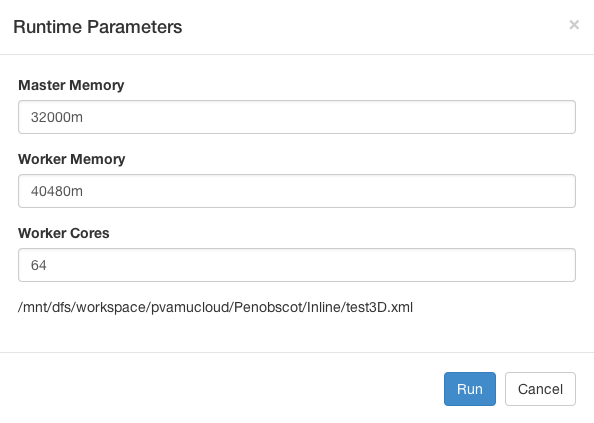
\includegraphics[scale=.60]{figures/Runtime.png}
\caption{Specify Runtime Parameters}
\label{Runtime}
\end{figure}
%%%%%%%%%%%%%%%%%%%%%%%%%%%%%%%%%%%%%%%%%%%%%%%%%%%%%%


\ifx true false
%%%%%%%%%%%%%%%%%%%%%%%%%%%%%%%%%%%%%%%%%%%%%%%%%%%%%%
%A table example is going to follow.
\begin{table}[h]
\centering
\caption{Provided UFuncs by ScalaNLP Breeze}
%\begin{tabular}{|p{4cm} |p{8cm} |}
\begin{tabular}{||l|l||}
\hline
Elementwise UFuncs & \shortstack[l]{exp, log, log1p, sqrt, \\sin, cos, tan, asin, acos, atan,\\sinh, cosh, tanh, asinh, acosh, atanh, \\floor, ceil, round, rint, signum, \\abs, isOdd, isEven,sigmoid} \\ 
\hline
Operator UFuncs &  \shortstack[l]{OpAdd: a + b, OpSub: a - b, OpMulMatrix: a * b, \\OpMulScalar: a :* b, OpSolveMatrixBy: a \textbackslash\ b,\\ OpMulInner: a dot b, OpNeg: -a, OpEq: a :== b,\\OpNe: a :!= b, OpLT: a :\textless\ b, OpLTE: a :\textless= b,\\OpGT: a :\textgreater b, OpGTE: a :\textgreater= b, \\OpAnd: a \& b, OpOr: a \textbar\ b, OpNot: !a } \\
\hline
Reduction UFuncs & \shortstack[l]{sum, product, softmax, any, all, \\min, max, argmin, argmax, \\norm, normalize, argsort, argtopk, \\mean, variance, stddev, meanAndVariance }\\
\hline
\end{tabular}
\label{tab:BreezeUFuncs}
\end{table}
%%%%%%%%%%%%%%%%%%%%%%%%%%%%%%%%%%%%%%%%%%%%%%%%%%%%%%
\fi

\section{Case Study}
The main characteristics of SAC are productivity, performance, usability and scalability. To prove them, some typical applications in seismic data processing are selected to run on SAC. As for usability and productivity, we will show some codes snippet need to be implemented by end user. As for the performance, execution time of both sequential codes and parallel codes on Spark are compared to get speedup factor, and for scalability, we will configure the running environment with different cores and analyze changing of execution time. To cover more seismic applications, we select four kinds of test cases: Linear Algebra Functions, Transformation and Filter, Statistics Functions and Complicate Stencil Operation to show how to implement them on SAC.

\ifx true false
\begin{table}[h]
\caption{Running Time of Sequential Codes with Different Split}
\centering
\begin{tabular}{||c| c c c ||} 
 \hline
 Lines per Split & 12 Lines & 60 Lines & 300 Lines \\ [0.5ex] 
 \hline
 Calculator & 4027 & 4244 & 4613 \\ 
 Hilbert Filter & 7532 & 6257 & 6194 \\
 Histogram & 4858 & 5508 & 5246 \\
 \hline
 \hline
 Subvolume Size & 3x3x3 & 9x9x9 & 17x17x17 \\ [0.5ex] 
 \hline
 FFT & 1395 & 27563 & 596789 \\
 Jacobi & 5972 & 86466 & 463102 \\
 \hline
\end{tabular}
\label{table:CalcSpark}
\end{table}
\fi

\subsection{Linear Algebra Functions}
Linear Algebra should be the fundamental technology in scientific computation. Basic arithmetic operations are easy implemented on normal data, but for big data, the situation is totally different. There are already some commercial and free softwares such as MATLAB, GNU Octave and Seismic Toolkit listed in \cite{SeismicCalculator} etc.  that could support linear algebra functions to process seismic data. All these softwares are running on PC, so the performance is bad for handling big seismic data, and most of them even could not handle big data due to the memory limitation. SAC is mainly focus on handling big data, in which data is distributed on different nodes and run arithmetic functions in parallel. Linear algebra functions could be applied on element (pixel), vector(trace) or matrix(plane). For single pixel or sample defined by Float type in Scala, all built-in operator could be used on pixel data. The more convenient way to implement such algorithms on vector or matrix are use operators and operations provided by Breeze. For trace and line template in SAC, the data types of input and output are DenseVector and DenseMatrix. ScalaNLP Breeze provide many Universal Functions (UFunc) that can operate on scalars, vectors, matrices, counters with little effort \cite{BreezeUFunc}. All Elementwise UFuncs from scala.math such as exp, log and trigonometric functions etc., and Operator UFuncs such as basic arithmetic, equality and comparison and boolean operations could be applied to DenseVector and DenseMatrix.  

To implement any algorithms or models, either in sequential codes or parallel codes the first step is to define the data type of input and output. For most applications in seismic area, the input could be one or more 3D volume, and the output could be one or more new 3D volume or some statistics results. But in the view of algorithm, we need to define smaller grain size such as pixel, trace, line or sub-volume. For example, we want to get max value from two seismic data, then the minimum grain size should be pixel. If a canny filter with window size 5x5 need to use 24 neighbor pixels, the minimum grain size should be a sub plane with at least 5x5 size. If size of input split is larger minimum grain, then it need to be split into minimum size in algorithms or models. List \ref{ScalaCode2Line} shows the sample codes of template: one process two Inlines (DenseMatrix) and generate one output Inline (DenseMatrix), another one process two Traces (DenseVector) and compute the euclidean distance (Float). 

The volume size of seismic data may so large that could not be fully cached in memory, so in the sequential codes, the input data set also need to be split into small parts that could fit in main memory and be processed one by one and then save back into disk after each part finished. For parallel codes in MPI, one node need to be in charge of reading data and scatters small trunks of data to other worker processes, and gathers results from each process then it finished. For the parallel codes running in SAC on Spark, user selects the grain size of input and output at first, then only need to write piece of codes in template. The performance of parallel codes may be affected by algorithms, data distribution, number of cores, memory size on each node and speed of communication link etc. 

\lstset{language=Java,frame=single}
\begin{lstlisting}[float,caption=Sample codes of arighmetic operations on two datasets,label=ScalaCode2Line]
//DenseMatrix Example:
class LineApplication2 extends java.io.Serializable {
    def processLine(line1:DenseMatrix[Double],
                      line2:DenseMatrix[Double])
                      :DenseMatrix[Double] = {
        sqrt(line1*line1 + line2*line2); 
    }
}
//DenseVector Example:
class TraceApplication2 extends java.io.Serializable {
    def processTrace(trace1:DenseVector[Double],
                       trace2:DenseVector[Double])
                       :Double = {
        sqrt(sum((trace1-trace2)*(trace1-trace2))); 
    }
}
\end{lstlisting}

\ifx true false
% put performance index of calculactor here.     
\begin{table}[h]
\caption{Running Time of Calculator on Spark with Different Configurations}
\centering
\begin{tabular}{||c| c c c c ||} 
 \hline
 Split & 72 Cores & 144 Cores & 288 Cores & 576 Cores \\ [0.5ex] 
 \hline
 1 & 915 & 740 & 722 & 724 \\ 
 10 & 212 & 177 & 216 & 442 \\
 30 & 278 & 304 & 387 & 502 \\
 100 & 493 & 453 & 471 & 827 \\
 \hline
\end{tabular}
\label{table:CalcSpark}
\end{table}
\fi

\subsection{Fourier \& Hilbert Transformation}
In signal and image processing, Fourier Transform (FT) is the most commonly used algorithm. The signal in time domain was decomposed into a series of frequencies  through FT, and in the frequency domain, many problems such as filter are easier to perform comparing with in the time domain. Fast Fourier transform (FFT) \cite{FFTWiki} is an algorithm to compute the discrete Fourier transform (DFT) and its inverse by factorizing the DFT matrix into a product of sparse (mostly zero) factors. There are different implementations of FFT, such as FFTW, OpenCV, Kiss FFT, Breeze etc. FFTW \cite{FFTW05} emphasizes performance by adapting to the hardware such as SIMD instructions in order to maximize performance, while Breeze aims to be generic, clean and powerful without sacrificing (much) efficiency. Breeze provide more concise interfaces of 1D/2D Fourier transforms and filtering functions, so we use FFT function in Breeze as test case by applying it both in sequential codes and parallel codes running on Spark. In this test case, the input of FFT is sub-volume of each pixel with its neighbors, which could be 3x3x3 or 9x9x9 and will be changed into a 1D array trace by trace. After applied FFT on such 1D array, the max value of FFT result will be saved to the center position in new volume. To implement it in SAC, user needs to define size of sub-volume, then writes FFT codes snippet inside template, in which type of input is Array[Float] and the one of output is Float.   

The Hilbert transform \cite{HilbertWiki} is important in the field of signal processing where it is used to derive the analytic representation of a signal. A great number of geophysical applications consists in close relation of the Hilbert transform to analytic functions of complex variable \cite{HilbertGeoApplication}. Hilbert transform approach now forms the basis by which almost all amplitude, phase and frequency attributes are calculated by ��current seismic interpretation softwares \cite{HilbertSeismic}. JTK already provided the Hilbert transform filter class, so we use it as test case by apply Hilbert transform filter on each trace of input seismic data set. In this template, the data type of input and output are both DenseVector[Float].  

Since the FFT and Hilbert transformation are both computation intensive, we will compare performance of sequential codes on single node with the one of parallel codes running in SAC on Spark with different configuration of memory and cores. Table \ref{table:HilbertSpark} shows the execution time of Hilbert transformation filter in both sequential codes and parallel codes on SAC. The same ones of FFT are shown in Table \ref{table:FFTSpark}. 

%put performance data of FFT and HTF here.

\begin{table}[h]
\caption{Running Time of Hilbert Transformation Filter on Spark with Different Configurations}
\centering
\begin{tabular}{||c| c c c c ||} 
 \hline
 Spark codes  & 72 Cores & 144 Cores & 288 Cores & 576 Cores \\ [0.5ex] 
 \hline
  Split 1   & 5947 & 3312 & 2004 & 1854 \\
  Split 10  & 5230 & 2746 & 1646 & 1628 \\
  Split 30  & 5260 & 2984 & 1839 & 1740 \\
  Split 100 & 5328 & 3357 & 2425 & 2517 \\
 \hline
 \hline
 Seq. codes & \multicolumn{4}{c||}{Average time is 6661} \\ 
 \hline
\end{tabular}
\label{table:HilbertSpark}
\end{table}

\begin{table}[h]
\caption{Running Time of FFT on Spark with Different Configurations}
\centering
\begin{tabular}{||c| c c c c ||} 
 \hline
 Spark Codes & 72 Cores & 144 Cores & 288 Cores & 576 Cores \\ [0.5ex] 
 \hline
 Subvolume 3x3x3 & 1229 & 687 & 570 & 562 \\ 
 Subvolume 9x9x9 & 22480 & 10101 & 6641 & 6850 \\ 
 \hline
 \hline
 Seq. codes of 3x3x3 & \multicolumn{4}{c||}{Average time is 83700 } \\ 
 \hline
 \end{tabular}
 \label{table:FFTSpark}
 \end{table}

\subsection{Statistics functions}
Descriptive statistics is the basis for data analytics, and in seismic data processing, most of statistical functions were already widely used. Spark itself provides some basic reduce functions (also called Actions) such as mean, variance, standard deviation and histogram on RDDs. Besides such basic statistical functions, Breeze also provides a fairly large number of probability distributions used for statistics signal processing. In this test, we use histogram as test case: the sequential codes will iterate whole data samples one by one in two loops, and parallel codes will use built-in histogram function in Spark. In the sequential codes of histogram, the min/max values are computed to define bucket array at first round, then each value is put into its related bucket in second iteration. The theory of histogram is same on Spark, but it was implemented by reduce and map functions on RDD.  Table \ref{table:HistSpark} shows the execution time of histogram in both sequential codes and parallel codes on SAC. 

%put performance of Histogram here.   

\begin{table}[h]
\caption{Running Time of Histogram on Spark with Different Configurations}
\centering
\begin{tabular}{||c| c c c c ||} 
 \hline
 Spark codes & 72 Cores & 144 Cores & 288 Cores & 576 Cores \\ 
 \hline
  Split 1   & 100  & 64   & 50   & 46   \\
  Split 10  & 216  & 326  & 466  & 639  \\
  Split 30  & 868  & 903  & 819  & 2113 \\
  Split 100 & 1802 & 1766 & 9244 & 8491 \\
 \hline
 \hline
 Seq. codes & \multicolumn{4}{c||}{Average time is 5204} \\ 
 \hline
\end{tabular}
\label{table:HistSpark}
\end{table}

\subsection{Complicate Stencil Operation}

Stencil codes are most common computations used in seismic image processing and reservoir simulation in oil \& gas industry, and most of codes in this domain are written in MPI or OpenMP programming models that running on huge clusters. But MPI codes involve more complexity of programming and could not handle fault tolerance very well, and although OpenMP make it easy to parallelize sequential codes, but with increasing size of volume of seismic data, SMP will encounter problem of caching large data and performance issue for data partition. 
We choose Scala as programming language for experiments and develop three applications: Sequential codes, Parallel codes using broadcasting variable and Parallel codes with boundary RDD. For the Sequential codes, we just split the big data file into small partition and each partition include several inlines, then using 3 nested loops to compute average value of 26 neighbor samples. After computation, results of each partition will be saved into file to be used as input for next iteration. For the Parallel codes with broadcasting variable, the large input dataset is distributed to all active nodes in whole cluster as RDD, then each node could get its own data section and apply map function(computation part) on it. Since boundary data is need for Jacobi kernel and there is no communication interfaces between mappers, the boundary Inlines of each split are collected as a big variable and broadcasted to all nodes by driver node after one iteration, then each node could fetch new boundary Inlines in next iterative computation. After implementation of Parallel codes using broadcasting variable, we found the performance of collecting data is very bad, so we design new Parallel codes using Cassandra DB and boundary RDDs to exchange boundary data and to avoid collecting data in each iteration. 

The data flow of two parallel methods (broadcast variables and boundary RDD) are shown in Figure \ref{JacobiCode}: Each number denotes one Inline of seismic data. The big seismic data files are stored on HDFS, which will be divided into small partitions and send to each node by driver node. Using broadcast variables shown in top half of diagram, the driver node needs to collect boundary Inlines from every node, which will take more time on network communication. The solution of using boundary RDDs is shown in below half diagram, in which boundary RDDs is filtered from result RDD, but they need repartition and resort for alignment and then merge with original RDD to form new RDD for next iteration. In the programmer view of sharing data, sharing with Cassandra database is similar to broadcast variables of Spark, but the underline data communication is distinct. Table \ref{table:JacobiSpark} shows the execution time of Jacobi computation in both sequential codes and parallel codes of 3 methods on SAC. 

%%%%%%%%%%%%%%%%%%%%%%%%%%%%%%%%%%%%%%%%%%%%%%%%%%%%%%%
\begin{figure}[h]
\centering
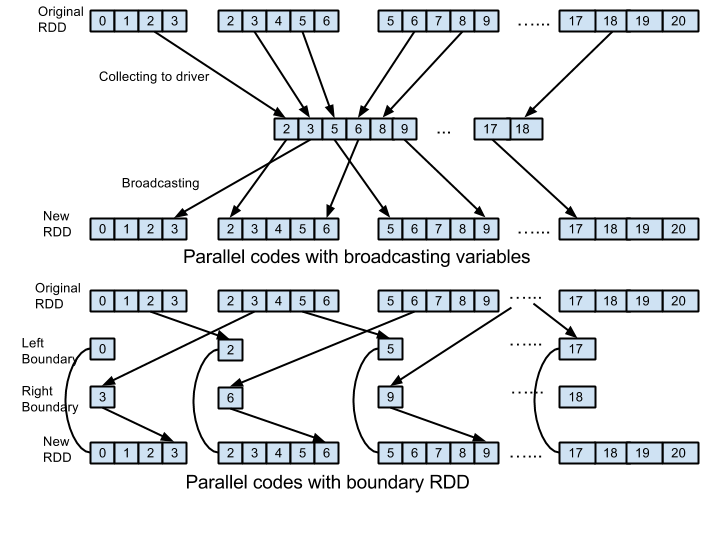
\includegraphics[scale=.6]{figures/JacobiCode.png}
\caption{Data Flow of Jacobi Parallel Codes}
\label{JacobiCode}
\end{figure}
%%%%%%%%%%%%%%%%%%%%%%%%%%%%%%%%%%%%%%%%%%%%%%%%%%%%%%

%put performance of Jacobi here.   

\begin{table}[H]
\caption{Running Time of Jacobi on Spark with Different Configurations}
\centering
\begin{tabular}{||c| c c c c ||} 
 \hline
 Spark codes & 72 Cores & 144 Cores & 288 Cores & 576 Cores \\ [0.5ex] 
 \hline
 Broadcast Var. & 1384 & 1908 & 1928 & 2239 \\ 
 Cassandra DB   & 701  & 508  & 409  & 398  \\
 Boundary RDD   & 196  & 158  & 146  & 150  \\
 \hline
 \hline
 Seq. codes & \multicolumn{4}{c||}{Average time is 5972} \\ 
 \hline
\end{tabular}
\label{table:JacobiSpark}
\end{table}

